\documentclass{article}
\setlength{\parskip}{0pt} % esp. entre parrafos
\setlength{\parindent}{3pt} % esp. al inicio de un parrafo
\usepackage{amsmath} % mates
\usepackage{listings}
\usepackage[sort&compress,numbers]{natbib} % referencias
\usepackage{url} % que las URLs se vean lindos
\usepackage[top=10mm,left=20mm,right=20mm,bottom=25mm]{geometry} % \textbf{\textbf{}}margenes
\usepackage{hyperref} % ligas de URLs
\usepackage{graphicx} % poner figuras
\usepackage[spanish]{babel} % otros idiomas
\hypersetup{
    colorlinks=true,
    linkcolor=blue,
    filecolor=blue,      
    urlcolor=blue,
    citecolor=black,
}

\title{TAREA \# 6 \\ Sistema multiagente} %titulo
\author{Natalia Berenice P\'{e}rez L\'{o}pez} % author
\date{\today}

\begin{document} % inicia contenido

\maketitle % cabecera

\section{Objetivo}
El objetivo de esta práctica es primero vacunar con probabilidad $p_v$ a los agentes al momento de crearlos, de tal forma que estén desde el inicio en el estado $R$, lo cual indica que ya no podrían contagiarse ni propagar la infección. Después se debe estudiar el efecto estadístico del valor de $p_v$ en (de cero a uno en pasos de $0.1$) el porcentaje máximo de infectados durante la simulación y el momento (iteración) en el cual se alcanza ese máximo.

\section{Desarrollo} % seccion y etiqueta
Para generar el código objetivo de esta práctica se realizaron algunas ideas y pruebas iniciales del código, las cuales se encuentran en \href{https://github.com/nataliaperez0/Simulation/tree/main/Tarea6}{mi repositorio}  en GitHub. Se inició tomando como base el código revisado en clase \citep{1} para calcular el movimiento de los agentes, los contagios y los agentes recuperados. Las modificaciones que se le realizaron a este código fueron; agregar un ciclo \texttt{for} para variar la probabilidad de vacunación ($p_v$) en pasos de $0.1$ desde cero a uno, vacunar desde el inicio a los agentes de acuerdo a la probabilidad $p_v$, agregar otro ciclo \texttt{for} para hacer $12$ réplicas para cada $p_v$, agregar un condicional \texttt{if} para generar las gráficas del movimiento de los agentes solamente para la primer réplica de cada $p_v$ y generar un \texttt{data.frame} que contiene la probabilidad de vacunación, el número de réplica, el número máximo de agentes infectados por réplica y el número de iteración en el que sucede este máximo. A continuación se muestra el código modificado para esta práctica: 
\bigskip

\definecolor{verde}{rgb}{0,0.56,0.22}
\definecolor{codegray}{rgb}{0.5,0.5,0.5}
\definecolor{codegreen}{rgb}{0,0.56,0.22}
\definecolor{backcolour}{rgb}{0.95,0.95,0.92}
\definecolor{azul}{rgb}{0,0,1}

\lstdefinestyle{mystyle}{
    backgroundcolor=\color{backcolour},   
    commentstyle=\color{verde},
    keywordstyle=\color{azul},
    numberstyle=\tiny\color{codegray},
    stringstyle=\color{codegreen},
    basicstyle=\ttfamily\footnotesize,
    breakatwhitespace=false,         
    breaklines=true,                 
    captionpos=b,                    
    keepspaces=true,                 
    numbers=left,                    
    numbersep=5pt,                  
    showspaces=false,                
    showstringspaces=false,
    showtabs=false,                  
    tabsize=2
}

\lstset{style=mystyle}
\begin{lstlisting}[language=R, caption= Código objetivo de la práctica para obtener la cantidad máxima de infectados por replica y la iteración en la que ocurre.]
library(dplyr)
l <- 1
n <- 50
pi <- 0.05
pr <- 0.02
v <- l / 20
pv = seq(0, 1, 0.1)
replicas = 12
datos = data.frame()
infect <- c()

for (va in pv){
  for (rep in 1:replicas){
    agentes <- data.frame(x = double(), y = double(),
                          dx = double(), dy = double(),
                          estado  = character())
    for (i in 1:n) {
      e <- "S"
      if (runif(1) < pi) {
        e <- "I"
      }else {
        if(runif(1) < va){
          e = "R"
        }
      }
      agentes <- rbind(agentes, data.frame(x = runif(1, 0, l),
                                           y = runif(1, 0, l),
                                           dx = runif(1, -v, v),
                                           dy = runif(1, -v, v),
                                           estado = e, vacuna = va))
    }
    print(agentes)
    levels(agentes$estado) <- c("S", "I", "R")
    epidemia <- integer()
    r <- 0.1
    tmax <- 100
    digitos <- floor(log(tmax, 10)) + 1
    for (tiempo in 1:tmax) {
      infectados <- dim(agentes[agentes$estado == "I",])[1]
      epidemia <- c(epidemia, infectados)
      if (infectados == 0) {
        break
      }
      contagios <- rep(FALSE, n)
      for (i in 1:n) { # posibles contagios
        a1 <- agentes[i, ]
        if (a1$estado == "I") { # desde los infectados
          for (j in 1:n) {
            if (!contagios[j]) { # aun sin contagio
              a2 <- agentes[j, ]
              if (a2$estado == "S") { # hacia los susceptibles
                dx <- a1$x - a2$x
                dy <- a1$y - a2$y
                d <- sqrt(dx^2 + dy^2)
                if (d < r) { # umbral
                  p <- (r - d) / r
                  if (runif(1) < p) {
                    contagios[j] <- TRUE
                  }
                }
              }
            }
          }
        }
      }
      for (i in 1:n) { # movimientos y actualizaciones
        a <- agentes[i, ]
        if (contagios[i]) {
          a$estado <- "I"
        } else if (a$estado == "I") { # ya estaba infectado
          if (runif(1) < pr) {
            a$estado <- "R" # recupera
          }
        }
        a$x <- a$x + a$dx
        a$y <- a$y + a$dy
        if (a$x > l) {
          a$x <- a$x - l
        }
        if (a$y > l) {
          a$y <- a$y - l
        }
        if (a$x < 0) {
          a$x <- a$x + l
        }
        if (a$y < 0) {
          a$y <- a$y + l
        }
        agentes[i, ] <- a
      }
      aS <- agentes[agentes$estado == "S",]
      aI <- agentes[agentes$estado == "I",]
      aR <- agentes[agentes$estado == "R",]
      resultado = c(va, rep, tiempo)
      datos = rbind(datos, resultado)
      names(datos) = c("Vacuna", "Replica", "Iteracion")
      tl <- paste(tiempo, "", sep="")
      vl = paste(va, "", sep="")
      while (nchar(tl) < digitos) {
        tl <- paste("0", tl, sep="")
        vl = paste("0", vl, sep="")
      }
      if (rep == 1){
        salida <- paste("p6_t", vl, tl, ".png", sep="")
        tiempo <- paste("Paso", tiempo)
        png(salida)
        plot(l, type="n", main=c(tiempo, va), xlim=c(0, l), ylim=c(0, l), xlab="x", ylab="y")
        if (dim(aS)[1] > 0) {
          points(aS$x, aS$y, pch=15, col="chartreuse3", bg="chartreuse3")
        }
        if (dim(aI)[1] > 0) {
          points(aI$x, aI$y, pch=16, col="firebrick2", bg="firebrick2")
        }
        if (dim(aR)[1] > 0) {
          points(aR$x, aR$y, pch=17, col="goldenrod", bg="goldenrod")
        }
        graphics.off()
      }
    }
    #salida <- paste("Vacuna=", va, ".png", sep="")
    #png(salida)
    #plot(1:length(epidemia), 100 * epidemia / n, xlab="Tiempo", ylab="Porcentaje de infectados",
    #main=paste("Vacunados:",va * 100, "%"))
    #graphics.off()
    infect <- c(infect, epidemia)
  }
}

datos2 <- data.frame(Cantidad_infectados = c(infect))
datos2 <- filter(datos2, Cantidad_infectados > 0)
New = cbind(datos, datos2)
MaxInfectados <- New %>% 
  group_by(Vacuna, Replica) %>%
  filter(Cantidad_infectados == max(Cantidad_infectados))

MaxInfectados2 <- MaxInfectados %>% 
  group_by(Vacuna, Replica) %>%
  filter(Iteracion == min(Iteracion))

library(ggplot2)
MaxInfectados2$Vacuna = as.factor(MaxInfectados2$Vacuna)
ggplot(MaxInfectados2, aes(x= Vacuna, y= Iteracion, fill = Vacuna)) + 
  geom_boxplot()+
  labs(x = "Probabilidad de vacuna", y = "Iteracion")

ggplot(MaxInfectados2, aes(x= Vacuna, fill = Vacuna, y = ((Cantidad_infectados/50) * 100))) + 
  geom_boxplot()+
  labs(x = "Probabilidad de vacuna", y = "Mayor porcentaje de infectados")
\end{lstlisting}

Para analizar los resultados obtenidos primero se graficó en un diagrama caja-bigote la cantidad máxima de agentes infectados en porcentaje para cada $p_v$ (Ver figura \ref{Figura1}). En este diagrama podemos ver que entre mayor sea la probabilidad de vacunación de los agentes se tienen menos infectados, lo cual es un dato coherente ya que cuando el agente está vacunado no puede contagiarse ni propagar la infección. 
\bigskip

Otro dato importante de analizar en el experimiento es el tiempo o iteración en el cual se tiene la mayor cantidad de agentes infectados, ya que en la vida real esta iteración podría representar por ejemplo el $pico$ de una pandemia, por lo tanto nos interesaría retardar la presencia de este $pico$ para preparar adecuadamente las instalaciones hospitalarias y así poder enfrentar la pandemia. Para analizar las iteraciones se realizó otro diagrama caja-bigote, el cual se muestra en la figura \ref{Figura2}, en este diagrama podemos ver que al aumentar la probabilidad de vacunación de los agentes se consigue alcanzar un número de iteración mayor, esto se mantiene hasta la $p_v$ de $0.8$ ya que después de esta se alcanzan iteraciones menores. Es importante mencionar que en la figura \ref{Figura2} se está graficando la primera iteración en la que se tiene el mayor porcentaje de agentes infectados, ya que este mayor porcentaje puede continuar varias iteraciones más y después disminuir su valor.
\bigskip

Para analizar si existe una relación entre la variación de la probabilidad de vacunación de los agentes y la cantidad mayor de agentes infectados se realizó una prueba estadística. Primero se elegió utilizar la prueba estadística ANOVA de una vía, pero debido a los resultados obtenidos al revisar la normalidad de los datos, se eligió realizar la prueba estadística \texttt{Kruskal Wallis} \citep{2}.
\bigskip

\newpage

\begin{figure} [h!]% figura
    \centering
    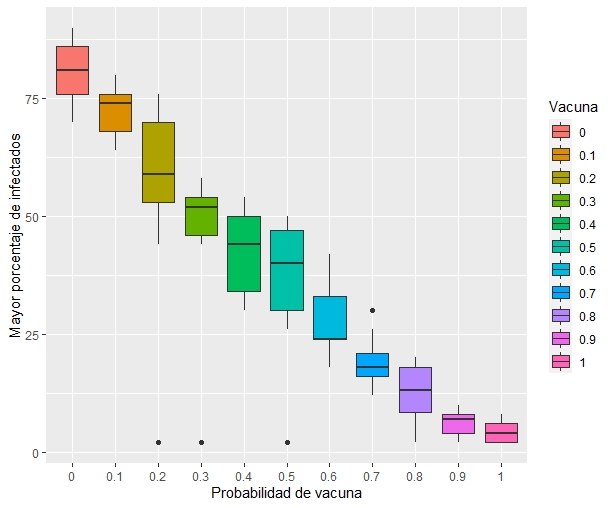
\includegraphics[width=129mm]{Figura1.jpeg} % archivo
    \caption{Mayor porcentaje de agentes infectados por replica para cada probabilidad de vacunación $p_v$.}
    \label{Figura1}
\end{figure}

\begin{figure} [h!]% figura
    \centering
    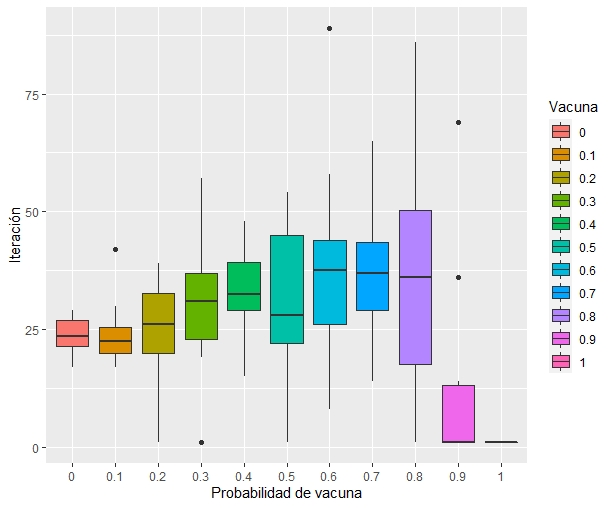
\includegraphics[width=129mm]{Figura2.jpeg} % archivo
    \caption{Iteración donde se presenta el máximo número de agentes infectados para cada $p_v$.}
    \label{Figura2}
\end{figure}

\bigskip
En el cuadro \ref{Cuadro1} se  resumen los resultados de la revisión de los supuestos para poder aplicar la prueba estadística. El supuesto outliers se refiere a la cantidad de valores atípicos que existen en los grupos, la normalidad por grupos se obtuvo con la prueba de \texttt{Shapiro Wilk}.

\begin{table}[ht]
\centering
\caption{Resultados del los supuestos para aplicar la prueba estadística.}
\smallskip

\begin{tabular}{ |p{2.1cm}|p{10.5cm}|}
 \hline
 Outliers & $4$ \\
 \hline
 Normalidad por grupo & $0$: $p$ = $0.550$ / $0.1$: $p$ = $0.449$ / $0.2$: $p$ = $0.007$ / $0.3$: $p$ = $4.31\times 10^{-5}$ $0.4$: $p$ = $0.085$ / $0.5$: $p$ = $0.040$ / $0.6$: $p$ = $0.146$ / $0.7$: $p$ = $0.626$ / $0.8$: $p$ = $0.453$ / $0.9$: $p$ = $0.126$ / $1$: $p$ = $0.033$\\
 \hline
 Normalidad & $p$ = $3.64\times 10^{-6}$ \\
 \hline
\end{tabular}
\label{Cuadro1}
\end{table}

En los resultados se observa que para la normalidad por grupos existen valores de $p$ menores a $0.05$, y la normalidad general de todo el conjunto de datos es de $p < 0.05$, por lo tanto no se tiene normalidad, así que es necesario realizar la prueba estadística \texttt{Kruskal Wallis} ya que ésta es útil para cuando no se tiene normalidad en los grupos de datos.
\bigskip

Al realizar la prueba \texttt{Kruskal Wallis} se obtienen los resultados mostrados en el cuadro \ref{Cuadro2}.

\begin{table}[ht]
\centering
\caption{Resultados al aplicar la prueba estadística \texttt{Kruskal Wallis}.}
\smallskip

\begin{tabular}{ |p{2.1cm}|p{2.1cm}|}
 \hline
 Chi cuadrada & Valor de $p$ \\
 \hline
 $105.96$ & $2.2\times 10^{-16}$ \\
 \hline
\end{tabular}
\label{Cuadro2}
\end{table}

Hipótesis nula : Las medias son iguales en todos los grupos.
\smallskip

Hipótesis alternativa: Debido a que $p < 0.05$ se rechaza la hipótesis nula, es decir que si existen diferencias significativas entre las medias de los grupos. 
\smallskip

Se entiende entonces que la variación de la probabilidad de vacunación de los agentes si tiene un efecto significativo en la cantidad máxima de infectados que se tendrán en cada réplica.
\bigskip

También podemos realizar la prueba de suma de rangos de \texttt{Wilcoxon} por pares \citep{4} para observar los resultados de $p$ y determinar si existen diferencias al comparar entre ellas cada una de las probabilidades de vacunación (Ver cuadro \ref{Cuadro3}).

\begin{table}[ht]
\centering
\caption{Resultados al aplicar la prueba \texttt{Wilcoxon}.}
\smallskip

\begin{tabular}{|p{1.7cm}|p{1cm}|p{1cm}|p{1cm}|p{1cm}|p{1cm}|p{1cm}|p{1cm}|p{1cm}|p{1cm}|p{1cm}|}
 \hline
Valor de $p$ & $0$ & $0.1$ & $0.2$ & $0.3$ & $0.4$ & $0.5$ & $0.6$ & $0.7$ & $0.8$ & $0.9$\\
 \hline
 $0.1$ & $0.0624$ & - & - & - & - & - & - & - & - & -\\
 \hline
 $0.2$ & $0.0056$ & $0.0499$ & - & - & - & - & - & - & - & -\\
 \hline
 $0.3$ & $0.0022$ & $0.0022$ & $0.1512$ & - & - & - & - & - & - & - \\
 \hline
 $0.4$ & $0.0017$ & $0.0017$ & $0.0494$ & $0.1849$ & - & - & - & - & - & - \\
 \hline
 $0.5$ & $0.0022$ & $0.0022$ & $0.0309$ & $0.1094$ & $0.3056$ & - & - & - & - & - \\
 \hline
 $0.6$ & $0.0017$ & $0.0017$ & $0.0140$ & $0.0194$ & $0.0252$ & $0.1120$ & - & - & - & - \\
 \hline
 $0.7$ & $0.0022$ & $0.0022$ & $0.0178$ & $0.0239$ & $0.0024$ & $0.0309$ & $0.0580$ & - & - & - \\
 \hline
 $0.8$ & $0.0028$ & $0.0028$ & $0.0194$ & $0.0252$ & $0.0028$ & $0.0252$ & $0.0053$ & $0.1512$ & - & - \\
 \hline
 $0.9$ & $0.0017$ & $0.0017$ & $0.0126$ & $0.0178$ & $0.0017$ & $0.0178$ & $0.0017$ & $0.0021$ & $0.1094$ & - \\
 \hline
 $1$ & $0.0017$ & $0.0017$ & $0.0087$ & $0.0131$ & $0.0017$ & $0.0131$ & $0.0017$ & $0.0021$ & $0.0252$ & $0.1848$ \\
 \hline
\end{tabular}
\label{Cuadro3}
\end{table}

En los resultados de la prueba podemos observar que la mayoría de los valores de $p$ son menores a $0.05$, solo existen algunas excepciones en las cuales se tiene una $p > 0.05$ como por ejemplo en la $p_v = 0.5$ comparada con la $p_v = 0.4$, lo cual indica que entre ellas no existen diferencias significativas en sus medias.
\bigskip

Posteriormente, para analizar estadísticamente los resultados mostrados en la figura \ref{Figura2} también se realizó la prueba estadística \texttt{Kruskal Wallis}. En el cuadro \ref{Cuadro4} se  resumen los resultados de la revisión de los supuestos para poder aplicar la prueba estadística. El supuesto outliers se refiere a la cantidad de valores atípicos que existen en los grupos, la normalidad por grupos se obtuvo con la prueba de \texttt{Shapiro Wilk}.
\newpage

\begin{table}[ht]
\centering
\caption{Resultados del los supuestos para aplicar la prueba estadística.}
\smallskip

\begin{tabular}{ |p{2.1cm}|p{3cm}|}
 \hline
 Outliers & $5$ \\
 \hline
 Normalidad & $p$ = $1.82\times 10^{-5}$ \\
 \hline
\end{tabular}
\label{Cuadro4}
\end{table}

En los resultados se observa que el valor de $p$ es menor a $0.05$, por lo tanto no se tiene normalidad. Al realizar la prueba \texttt{Kruskal Wallis} se obtienen los resultados mostrados en el cuadro \ref{Cuadro5}.

\begin{table}[ht]
\centering
\caption{Resultados al aplicar la prueba estadística \texttt{Kruskal Wallis}.}
\smallskip

\begin{tabular}{ |p{2.1cm}|p{2.1cm}|}
 \hline
 Chi cuadrada & Valor de $p$ \\
 \hline
 $49.99$ & $2.67\times 10^{-7}$ \\
 \hline
\end{tabular}
\label{Cuadro5}
\end{table}

Hipótesis nula : Las medias son iguales en todos los grupos.
\smallskip

Hipótesis alternativa: Debido a que $p < 0.05$ se rechaza la hipótesis nula, es decir que si existen diferencias significativas entre las medias de los grupos. 
\smallskip

Se entiende entonces que la variación de la probabilidad de vacunación de los agentes si tiene un efecto significativo en el número de iteración en la cual se presenta la cantidad máxima de agentes infectados.
\bigskip

Realizando la prueba de suma de rangos de \texttt{Wilcoxon} podemos observar los resultados de $p$ y determinar si existen diferencias al comparar entre ellas cada una de las probabilidades de vacunación (Ver cuadro \ref{Cuadro6}).

\begin{table}[ht]
\centering
\caption{Resultados al aplicar la prueba \texttt{Wilcoxon}.}
\smallskip

\begin{tabular}{|p{1.7cm}|p{1cm}|p{1cm}|p{1cm}|p{1cm}|p{1cm}|p{1cm}|p{1cm}|p{1cm}|p{1cm}|p{1cm}|}
 \hline
Valor de $p$ & $0$ & $0.1$ & $0.2$ & $0.3$ & $0.4$ & $0.5$ & $0.6$ & $0.7$ & $0.8$ & $0.9$\\
 \hline
 $0.1$ & $1$ & - & - & - & - & - & - & - & - & -\\
 \hline
 $0.2$ & $1$ & $1$ & - & - & - & - & - & - & - & -\\
 \hline
 $0.3$ & $1$ & $1$ & $1$ & - & - & - & - & - & - & - \\
 \hline
 $0.4$ & $0.4393$ & $0.8569$ & $1$ & $1$ & - & - & - & - & - & - \\
 \hline
 $0.5$ & $1$ & $1$ & $1$ & $1$ & $1$ & - & - & - & - & - \\
 \hline
 $0.6$ & $0.5930$ & $0.7066$ & $1$ & $1$ & $1$ & $1$ & - & - & - & - \\
 \hline
 $0.7$ & $0.4073$ & $0.8909$ & $1$ & $1$ & $1$ & $1$ & $1$ & - & - & - \\
 \hline
 $0.8$ & $1$ & $1$ & $1$ & $1$ & $1$ & $1$ & $1$ & $1$ & - & - \\
 \hline
 $0.9$ & $0.2295$ & $0.1959$ & $0.4308$ & $0.4073$ & $0.0963$ & $0.4073$ & $0.0963$ & $0.0914$ & $0.8569$ & - \\
 \hline
 $1$ & $0.0005$ & $0.0005$ & $0.0018$ & $0.0025$ & $0.0005$ & $0.0025$ & $0.0005$ & $0.0006$ & $0.0131$ & $0.5930$ \\
 \hline
\end{tabular}
\label{Cuadro6}
\end{table}

En los resultados de la prueba podemos observar que al comparar $p_v = 1$ con todas las demás $p_v$ siempre se obtienen valores de $p < 0.05$, lo cual indica que solamente con la probabilidad de vacunación de $1$ se tienen diferencias significativas en el número de iteración en la cual se presenta el máximo porcentaje de agentes infectados. 
\bigskip

A continuación se muestra el código utilizado para realizar las pruebas estadísticas \texttt{Kruskal Wallis}:

\lstset{style=mystyle}
\begin{lstlisting}[language=R, caption= Código para las pruebas estadísticas \texttt{Kruskal Wallis} y \texttt{Wilcoxon}.]
library(tidyverse)
library(ggpubr)
library(rstatix)
library(rapportools)
library(readr)

#PRUEBA ESTADISTICA PARA CANTIDAD DE INFECTADOS
#Estadisticas descriptivas
MaxInfectados2 %>%
  group_by(Vacuna) %>%
  get_summary_stats(Cantidad_infectados, type = "mean_sd")

#SUPUESTOS PARA ANOVA
#1:Outliers
MaxInfectados2 %>%
  group_by(Vacuna) %>%
  identify_outliers(Cantidad_infectados)

#2:Normalidad por Shapiro
MaxInfectados2 %>%
  group_by(Vacuna) %>%
  shapiro_test(Cantidad_infectados)

MaxInfectados2
str(MaxInfectados2)
names(MaxInfectados2)
shapiro.test(MaxInfectados2$Cantidad_infectados)

#PRUEBA ESTADISTICA KRUSKAL WALLIS
kruskal.test(Cantidad_infectados ~ Vacuna, data = MaxInfectados2)

#PRUEBA WILCOXON
pairwise.wilcox.test(MaxInfectados2$Cantidad_infectados, MaxInfectados2$Vacuna)

#PRUEBA ESTADISTICA PARA ITERACION
#Estadisticas descriptivas
MaxInfectados2 %>%
  group_by(Vacuna) %>%
  get_summary_stats(Iteracion, type = "mean_sd")

#SUPUESTOS PARA ANOVA
#1:Outliers
MaxInfectados2 %>%
  group_by(Vacuna) %>%
  identify_outliers(Iteracion)

#2:Normalidad por Shapiro
MaxInfectados2 %>%
  group_by(Vacuna) %>%
  shapiro_test(Iteracion)

MaxInfectados2
str(MaxInfectados2)
names(MaxInfectados2)
shapiro.test(MaxInfectados2$Iteracion)

#PRUEBA ESTADISTICA KRUSKAL WALLIS
kruskal.test(Iteracion ~ Vacuna, data = MaxInfectados2)

#PRUEBA WILCOXON
pairwise.wilcox.test(MaxInfectados2$Iteracion, MaxInfectados2$Vacuna)
\end{lstlisting}

\newpage
.
\bigskip

\section{Conclusi\'{o}n}
Con base en los diagramas caja-bigote y los resultados obtenidos de las pruebas estadísticas \texttt{Kruskal Wallis} y \texttt{Wilcoxon} puedo concluir que la variación de la probabilidad de vacunación de los agentes si afecta significativamente el máximo porcentaje de agentes infectados que se tendrá, ya que a mayor probabilidad $p_v$ se disminuye el porcentaje de agentes infectados. Además considero que la tasa más baja de vacunación para obtener la máxima cantidad de infectados en una iteración mayor es con una $p_v = 0.7$ o $p_v = 0.8$, ya que con estas probabilidades de vacunación se tiene un mayor porcentaje de infectados menor al 25\% de los agentes y además este porcentaje se puede presentar hasta iteraciones mayores a $50$, es decir que se podría posponer el $pico$ de la pandemia hasta la mitad de su duración total. 
\smallskip

En general ésta práctica fue de mi agrado porque nos muestra una aplicación en epidemiología, con la cual se puede representar adecuadamente la situación que se está viviendo en la actualidad con la pandemia del $Covid-19$. 
\newpage
.
\bigskip

\bibliography{referencias}
\bibliographystyle{plainnat}

\end{document}